\documentclass[11pt,a4paper]{article}
\usepackage{graphicx}
\usepackage{amssymb, amsmath}
\usepackage{url}
\usepackage{polski}
\usepackage{listings}
\usepackage{subfigure}
\usepackage[utf8]{inputenc} 

\title{Interpreter skryptów dla platformy Android OS\\ \large Projekt wstępny}
\author{Piotr Jastrzębski\\ \url{piotr.jastrzebski@gmail.com}}
\date{}
\begin{document}
\maketitle

\section{Opis funkcjonalności}
Projekt ma funkcjonować jako integralna część aplikacji, realizowanej na potrzeby pracy inżynierskiej. Będzie on działał pod kontrolą systemu Android, a napisany zostanie w Javie. W związku z koniecznością wielokrotnego testowania różnych funkcji aplikacji wektoryzacji obrazów bitmapowych z różnymi parametrami, interpreter powinien zapewnić taką możliwość, bez konieczności każdorazowej kompilacji. Wielokrotne wywołania mogą zostać wywołane skryptem z zastosowaniem pętli while, a parametry wywołań mogą być zależne od iteratora. Założeniem jest stworzenie interpretera obsługującego wczytywanie skryptów wywołań z poziomu interfejsu graficznego aplikacji. Skrypt powinien zostać przygotowany zgodnie z opisem i uwzględnieniem przeznaczenia zmiennych i wywołań podanymi w punkcie \ref{zmienne}. Gramatyka wywołań została przedstawiona w punkcie \ref{gramatyka}.

\subsection{Specyfikacja formalna}\label{zmienne}
Plik skryptowy dla aplikacji powinien być zapisany w formacie tekstowym z zachowaniem rozszerzenia pliku {\tt "txt"}, np. {\tt "skrypt.txt"}. Obecność białych znaków nie wpływa na działanie aplikacji. Poprawny skrypt musi zawierać wczytanie obrazu wzorcowego i zapis do pliku wyniku w postaci wektorowej. Zmienne liczbowe oraz ścieżka zapisu mogą być zależne od wartości zmiennej iteratora. Wartości argumentów funkcji uzależnić można poprzez dodanie wyrażenia {\tt +n} lub {\tt -n}, po liczbie, a do ścieżki poprzez dodanie {\tt +n+} przed rozszerzeniem pliku. (przyjmując, że {\tt n} wybrano jako symbol zmiennej) Poniżej przedstawiono listę przeznaczenia poszczególnych zmiennych wszystkich funkcji skryptu.
\begin{verbatim}
load(
   path           //bezwzględna ścieżka obrazu
)

hough_c(
   dp,            //odwrócony współczynnik proporcjonalności
                  //akumulatora
   minDist,       //minimalna odległość pomiędzy
                  //środkami okręgów
   gaussSize,     //rozmiar maski filtra Gaussa
   gaussSigma     //współczynnik sigma filtra Gaussa
)

hough_l(
   rho,           //rozdzielczość akumulatora w pikselach
   theta,         //rozdzielczość akumulatora w radianach
   threshold,     //wartość progowa akumulatora
   minLineLength, //minimalna długość odcinka
   maxLineGap,    //maksymalna długość przerwy
   cannyT1,       //mniejsza wartość progowa detektora Cannyego
   cannyT2        //większa wartość progowa detektora Cannyego
)

harris(
   maxCorners,    //maksymalna liczba zwracanych wierzchołków
   qualityLevel,  //minimalna "jakość" wierzchołka
   minDistance,   //minimalna odległość między zwracanymi
                  //wierzchołkami
   blockSize,     //rozmiar sąsiedztwa
   useHarris,     //korzysta z detektora Harrisa dla "true",
                  //dla "false" z cornerMinEigenVal() 
   k              //wolny parametr detektora Harrisa
)

save(
   path           //bezwzględna ścieżka rezultatu
)

while(
   var            //nazwa zmiennej (jedna litera)
   op             //relacja: <, >, <=, >=, ==, !=
   n              //wartość dziesiętna
)
{...}            //funkcje w pętli

ass(
   var,           //nazwa zmiennej (jedna litera)
   n              //przypisywana wartość (l. dziesiętna)
)

mod(              
   var,           //nazwa zmiennej (jedna litera)
   n              //zmiana wartości zmiennej (l. dziesiętna)
)

progress          //znacznik postępu
\end{verbatim}

\subsection{Składnia języka w notacji EBNF}\label{gramatyka} 
\begin{verbatim}
expression   = loadEx | saveEx | houghCEx | houghLEx |
               harrisEx | whileEx | assEx | modEx | progressEx;   
loadEx       = "load" , "("" , path , extensionIn , "")" ;
saveEx       = "save" , "("" , path , extensionOut , "")" ;
houghCEx     = "houghC" , "(" , d , n , n , n , ")" ;
houghLEx     = "houghL" , "(" , n , d , n , n ,
               n , n , n , ")" ;
harrisEx     = "harris" , "(" , n , d , n , n ,
               boolean , d , ")" ;
whileEx      = "while" , "(" , ( var | real ) , op ,
               ( var | real ) , ")" , "{" , {expression} , "}" ;
assEx        = "ass" , "(" , var , "," , real , ")" ;
modEx        = "mod" , "(" , var , "," , real , ")" ;
progressEx   = "progress" ;
path         = pathPart , { pathPart } ,
               [ "+" , var , +" ] , "." ;
pathPart     = "/" , ( character | digit ) , { character | digit } ;
extensionIn  = "jpg" | "jpeg" | "bmp" | "gif" | "png" ;
extensionOut = "svg" ;
n            = nat , varDep ;
d            = posReal , varDep ;
nat          = posDigit , {digit} | "0" ;
posReal      = nNum , [ "." , digit, {digit} ] ;
int          = [-] , nat ;
real         = [-] , posReal ;
varDep       = [ ( "-" | "+" ) , var ]
character    = var | "_" | "-" ;       
digit        = "0" | posDigit ;
var          = "a" | "b" | "c" | "d" | "e" | "f" | "g" |
               "h" | "i" | "j" | "k" | "l" | "m" | "n" |
               "o" | "p" | "q" | "r" | "s" | "t" | "u" |
               "v" | "w" | "x" | "y" | "z" ;
posDigit     = "1" | "2" | "3" | "4" | "5" | "6" | "7" |
               "8" | "9" ;
op           = "<" | ">" | "<=" | ">=" | "==" | "!=" ;                 
boolean      = "true" | "false" ;                  
\end{verbatim}

\section{Wymagania funkcjonalne}
\begin{itemize}
\item{parsowanie skryptów zapisanych w plikach tekstowych}
\item{umożliwienie wielokrotnego wykonywania wywołań zamkniętych w pętli while i zależnych od iteratora}
\item{przestrzeganie logicznego porządku wczytanie-funkcje-zapis}
\item{możliwość wywoływania funkcji wielokrotnie i w dowolnej kolejności}
\item{kontrola poprawności wprowadzonych danych}
\item{informowanie użytkownika, w którym miejscu skryptu wystąpił błąd}
\end{itemize}

\section{Wymagania niefunkcjonalne}
Projekt powstaje jako integralna część programu wektoryzacji obrazów bitmapowych realizowanego na potrzeby pracy inżynierskiej. Konieczne jest poszerzenie interfejsu użytkownika o dodatkowy przycisk wywołujący parsowanie skryptu. Ścieżkę do skryptu definiuje się w aktualnie istniejącym polu tekstowym aplikacji. Zrzuty ekranu z działania aplikacji przedstawiono na rysunku \ref{android}.

\section{Projekt realizacji}
Aplikacja parsera składa się z kilku modułów: skanera, parsera i analizatora składniowego. Schemat przekazywania informacji pomiędzy modułami, a także między elementami parsera a aplikacją wektoryzującą przedstawiono na rysunku \ref{schemat}. Tablica symboli jest tablicą globalną i przy wystąpieniu w strukturze skryptu nowego symbolu umieszcza go w strukturze tablicy. Symbole te wykorzystywane są potem podczas generacji i wykonywania kodu.
\\Klasy programu:
\begin{itemize}
\item \emph{StartActivity:} 	klasa UI (obsługa zdarzeń przycisków, przechwytywanie ścieżki skryptu, komunikacja z użytkownikiem)
\item \emph{FileUtil:} klasa obsługi pliku (obsługa plików, czytanie znaków ze strumienia)
\item \emph{ScanerUtil:} klasa skanera (rozbicie tekstu, pomijanie białych znaków, rozpoznawanie tokenów)
\item \emph{ParserUtil:} klasa parsera (tworzenie drzewa rozbioru, sprawdzanie zgodności z gramatyką)
\item \emph{SyntaxUtil:} klasa analizatora składniowego (sprawdzanie zgodności semantycznej skryptu z założeniami)
\item \emph{ProcessImage:} klasa przetwarzania obrazu (wykonuje funkcje graficzne na obrazie, zapisuje plik SVG)
\end{itemize}
\begin{figure}
\centering
\mbox{
\subfigure[Skrypt niepoprawny]{
\includegraphics[width=0.45\textwidth]{skrypt.png}}\quad
\subfigure[Skrypt poprawny]{
\includegraphics[width=0.45\textwidth]{skrypt2.png} }
}
\caption{Wygląd okna aplikacji w systemie Android}\label{android} 
\end{figure}
\begin{figure}
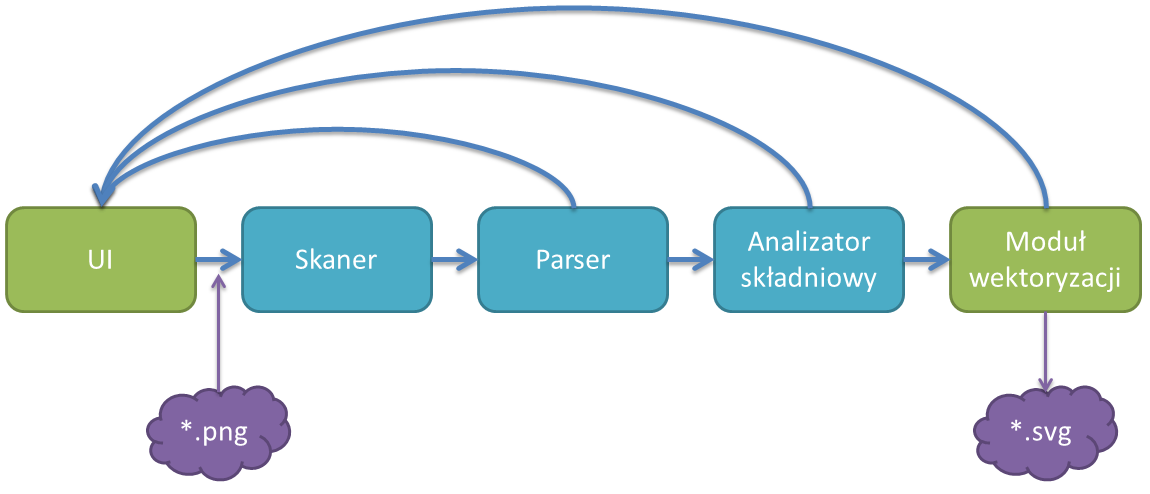
\includegraphics[width=\textwidth]{schemat.png}
\caption{Schemat zależności między modułami aplikacji.}
\label{schemat}
\end{figure}

\subsection{Analiza leksykalna (skanowanie)}
Polega na rozbiciu wczytanego z pliku tekstu na leksemy. Podczas skanowania ignorowane są wszelkie białe znaki. Następnie na podstawie leksemów zostają rozpoznane tokeny (odpowiednie przypasowanie do wzorca). Skaner rozpoznaje następujące tokeny:\\\\
\begin{tabular}{ | l | l | }
\hline                        
\bf{Przykład leksemu} & \bf{Token} \\\hline        
load & wyróżnik funkcji \\
save&\\
houghC&\\
houghL&\\
harris&\\
while&\\
mod&\\
ass&\\\hline
progress& znacznik postępu\\\hline
( & początek funkcji\\\hline
) & koniec funkcji\\\hline
\{ & początek pętli \\\hline
\} & koniec pętli \\\hline
- & minus \\\hline
, & przecinek\\\hline
x & zmienna\\\hline
!= & operator\\\hline
123 & liczba naturalna\\\hline
1.23 & liczba dziesiętna\\\hline
"/mnt/sdacrd/bsc/a.jpg" & napis\\\hline
true & wartość logiczna\\\hline
\end{tabular}
\\\\\\

Dla przykładu:
\begin{verbatim}
load("/mnt/sdcard/bsc/1.jpg")
harris(99, 0.01, 58, 3, true, 0.04)
save("/mnt/sdcard/bsc/w1.svg")
\end{verbatim}
analiza leksykalna wyglądałaby tak:
\begin{center}
\begin{tabular}{ | l | l | l | }
\hline                        
\bf{Leksem} & \bf{Token} & \bf{Atrybut} \\ \hline        
load & wyróżnik funkcji & load\\ \hline
(& początek funkcji & \\ \hline    
"/mnt/sdcard/bsc/1.jpg" & napis & /mnt/sdcard/bsc/1.jpg\\ \hline   
) & koniec funkcji &\\ \hline   
harris & wyróżnik funkcji & harris\\ \hline
(& początek funkcji & \\ \hline  
99 & liczba naturalna &99\\ \hline   
, & przecinek &\\ \hline   
0.01 & liczba dziesiętna &0.01\\ \hline   
, & przecinek &\\ \hline    
58 & liczba naturalna &58\\ \hline   
, & przecinek &\\ \hline   
3 & liczba naturalna &3\\ \hline   
, & przecinek &\\ \hline   
true & wartość logiczna & true\\ \hline   
, & przecinek &\\ \hline   
0.04 & liczba dziesiętna &0.04\\ \hline   
) & koniec funkcji &\\ \hline   
save & wyróżnik funkcji & save\\ \hline
( & początek funkcji & \\ \hline
"/mnt/sdcard/bsc/w1.svg" & napis & /mnt/sdcard/bsc/w1.svg\\ \hline   
) & koniec funkcji &\\ \hline   
\end{tabular}
\end{center}

\subsection{Analiza składniowa (parsowanie)}
Analizator składniowy (parser) otrzymawszy od skanera ciąg symboli leksykalnych sprawdza czy może on zostać wygenerowany przez gramatykę. Tworzone jest drzewo składni na podstawie zapytania i sprawdzana są możliwości wykonania zapytania. W przypadku niemożliwości wygenerowania parser zgłasza błąd, o którym informuje użytkownika i przerywa interpretację.
\\\\
Lista produkcji:
\begin{verbatim}
S         = wyróżnik funkcji + początek funkcji + ARGUMENTY
            + koniec funkcji
S         = wyróżnik funkcji + początek funkcji + WARUNEK
            + koniec funkcji + początek pętli + FUNKCJE
            + koniec pętli
S         = znacznik postępu
FUNKCJE   = S
FUNKCJE   = S + FUNKCJE
WARUNEK   = zmienna + operator + l. dziesiętna
WARUNEK   = zmienna + operator + minus + l. dziesiętna
ARGUMENTY = zmienna + przecinek + l. dziesiętna
ARGUMENTY = zmienna + przecinek + minus + l. dziesiętna
ARGUMENTY = napis
ARGUMENTY = l.dziesiętna + l.naturalna + l.naturalna + l.naturalna
ARGUMENTY = l.naturalna + l.dziesiętna +l.naturalna + l.naturalna
            + l.naturalna + l.naturalna + l.naturalna
ARGUMENTY = l.naturalna + l.dziesiętna + l.naturalna + l.naturalna
            + w.logiczna + l.naturalna
\end{verbatim}

Każdy symbol nieterminalny gramatyki odpowiada jednemu węzłowi w drzewie rozbioru. Każdy taki węzeł ma swoją metodę \emph{execute()}, która daje wynik po analizie wywołań funkcji \emph{execute()} węzłów podrzędnych itd.\\\\
Struktury danych:
\begin{itemize}
\item \emph{SAbstractC:} 	klasa abstrakcyjna węzła
\item \emph{SWhileC:}		klasa pętli while
\item \emph{SFunC:}		klasa funkcji innych niż pętla while
\item \emph{FunsC:}		klasa pozwalająca na hierarchiczne wywoływanie funkcji
\item \emph{ArgsC:}		klasa nadrzędna zbiorów argumentów
\item \emph{CondC:}		klasa warunku logicznego
\item \emph{NatC:}			klasa l. naturalnej
\item \emph{PosRealC:}		klasa l. rzeczywistej nieujemnej
\item \emph{BoolC:}		klasa w. logicznej
\item \emph{StringC:}		klasa napisu
\end{itemize}

\subsection{Analiza semantyczna}
Po zakończeniu faz analizy leksykalnej i analizy składniowej następuje analiza semantyczna. Zadaniem tej fazy jest sprawdzenie programu źródłowego pod względem semantycznej zgodności z definicją języka źródłowego np. czy typy operandów są zgodne z wymaganiami.

\section{Przykłady testowe}
\subsection{Pozytywne}
Powinny zrealizować wczytanie, zrealizowanie funkcji przetwarzania obrazów, a następnie zapisanie wyników wykrywania tych elementów w sposób wektorowy do pliku SVG:
\begin{itemize}

\item Wykrywanie okręgów, odcinków, wierzchołków.
\begin{verbatim}
load("/mnt/sdcard/bsc/1.jpg")
houghC(1.150, 58, 9, 2)
houghL(1, 0.0174532925, 10, 10, 10, 50, 200)
harris(99, 0.01, 58, 3, true, 0.04)
save("/mnt/sdcard/bsc/wynik_skrypt1.svg")
\end{verbatim}

\item Wykrywanie odcinków.
\begin{verbatim}
load("/mnt/sdcard/camera/DCIM1209.jpeg")
houghL(1, 0.02, 10, 5, 20, 75, 100)
save("/mnt/sdcard/test/test.svg")
\end{verbatim}
\end{itemize}
\subsection{Negatywne}
\begin{itemize}
\item Parser powinien zwrócić błąd dla:

\begin{verbatim}
load("/mnt/sdcard/bsc/1.jpg)     //brak domknięcia cudzysłowu
houghC(1.150, 58, 9)             //zbyt mała liczba argumentów
ass(xy, -12.3)                   //nieprawidłowa zmienna
xyz(99, 0.01, 58, 3, true, 0.04) //nieznana funkcja
save("/mnt/sdcard+x+/wynik.svg") //uzależnienie od zmiennej
                                 //w złym miejscu
\end{verbatim}
\end{itemize}
\end{document}
